%!TEX root = ../template.tex
%Developed using Sublime Text 3 with LaTexTools plugin
%SUPER+b for compiling latex to pdf
%Don't forget to use SUPER+R to jump between top level commands!
%F6 to spell check
%%%%%%%%%%%%%%%%%%%%%%%%%%%%%%%%%%%%%%%%%%%%%%%%%%%%%%%%%%%%%%%%%%%%
%% chapter4.tex
%% UNL thesis document file
%%
%% Chapter with the info about the available data
%%%%%%%%%%%%%%%%%%%%%%%%%%%%%%%%%%%%%%%%%%%%%%%%%%%%%%%%%%%%%%%%%%%%
\chapter{Proposed Approach}
\label{cha:available_data}
% ================
% = Introduction =
% ================

For this dissertation's work, it's proposed a CRISP-DM methodology to approach the problem. An explanation about this methodology is presented in section \ref{sec:crispdm}, following a suggested working plan for this dissertation in section \ref{sec:work_plan}. In section \ref{sec:available_data} the available data is presented and its quality is discussed, referring that an additional dataset is expected.

As off the time this document is being written, the Business Understanding phase has already finished and the current focus is on the Data Understanding and the Data Preparation.

\todo[inline]{colocar aqui o primeiro nivel de cada tarefa}

\todo[inline]{na parte de utilização das tecnicas, ser mencionado de forma suave o que é cada técnica}



\section{\Acrlong{crispdm}} % (fold)
\label{sec:crispdm}

\Acrfull{crispdm} is an iterative data mining process model that describes commonly used approaches that data mining experts use to tackle problems, which was developed by analysts representing Daimler-Chrysler, SPSS, and NCR. \Acrshort{crispdm} provides a nonproprietary and freely available standard process for fitting data mining into the general problem-solving strategy of a business or research unit.

In this methodology, a data mining project has a life-cycle consisting in six phases, where the next phase in the sequence often depends on the outcomes associated with the previous phase - making it an adaptive methodology, where the sequence of the phases is not strict and moving back and forth between different phases is always required.

The iterative nature of \Acrshort{crispdm} provides a continuous approach for cases when the solution to a particular business or research problem leads to further questions of interest, which may then be attacked using the same general process as before.


\begin{figure}[htbp]
	\centering
	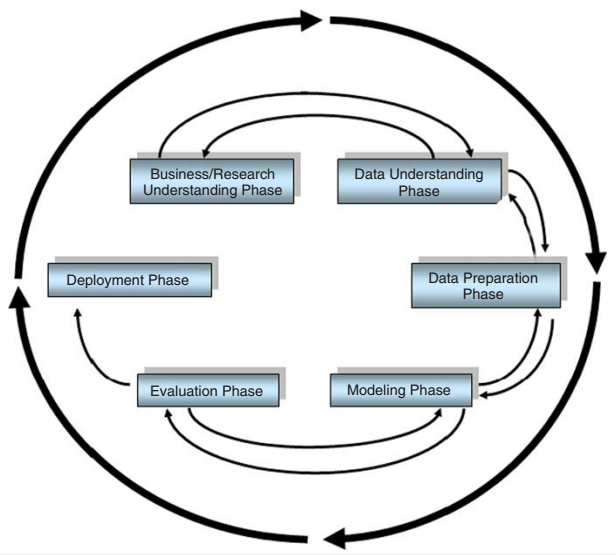
\includegraphics[width=4.5in ]{crispdm}
	\caption{\Acrshort{crispdm} process}
	\label{fig:crispdm}
\end{figure}

\subsection{\Acrshort{crispdm} phases}
\label{sec:crispdm_phases}

\subsubsection{Business/Research Understanding}

\subsubsection{Data Understanding}

\subsubsection{Data Preparation}

\subsubsection{Modeling}

\subsubsection{Evaluation}

\subsubsection{Deployment}

\section{Work Plan} % (fold)
\label{sec:work_plan}

\section{Available Data}
\label{sec:available_data}
